\documentclass[aspectratio=169,10pt]{beamer}

% localisation settings
\usepackage[utf8]{inputenc}
\usepackage[T1]{fontenc}
\usepackage[australian]{babel}
\usepackage{csquotes}

\usepackage{tikz}

\usepackage{color}

\usetikzlibrary{math,decorations.pathreplacing,calc,decorations.markings}
\usetikzlibrary{automata, positioning,fit,backgrounds}

\usepackage{framed}

\tikzset{->-/.style={decoration={
			markings,
			mark=at position {0.5*\pgfdecoratedpathlength+.5*3pt} with {\arrow{>}}},postaction={decorate}}}

\tikzset{-<-/.style={decoration={
			markings,
			mark=at position {0.5*\pgfdecoratedpathlength+.5*3pt} with {\arrow{<}}},postaction={decorate}}}


\usetheme{metropolis}
\usecolortheme{owl}
%\metroset{background=dark}
\metroset{block=fill}

\usefonttheme[onlymath]{serif}
\usepackage{parskip}

\usepackage{hyperref}

% citations
\usepackage[
	backend=biber,
	style=authoryear,
	safeinputenc,
	useprefix]{biblatex}

% make sure that names are not sorted by prefix first
\DeclareSortingNamekeyTemplate{
	\keypart{
		\namepart{family}}
	\keypart{
		\namepart{prefix}}
	\keypart{
		\namepart{given}}
	\keypart{
		\namepart{suffix}}
}
% make sure that the prefix is not capitalised
%  BibLaTeX will capitalise the first letter in some cases, this stops this
\renewbibmacro{begentry}{\midsentence}
\DeclareDelimFormat[bib]{nametitledelim}{\newline\bibsentence}
\renewbibmacro{in:}{\newline In:}
% make sure that biblatex uses a non-breaking space in \textcite
\renewcommand\namelabeldelim{\addnbspace}
\addbibresource{main.bib}
\usepackage{mathscinet} % support for additional accents

% math packages
\usepackage{amsfonts,amsmath,amsthm,amssymb,mathtools,stmaryrd,mathrsfs}
\usepackage{multirow}

\usepackage{ragged2e}
\justifying

\renewcommand{\leq}{\leqslant}
\renewcommand{\geq}{\geqslant}

%\newcommand\at{\mathrm{{\fontfamily{qbk}\selectfont\small @}}}
\newcommand\at{|_}

\author[A.~Bishop]{Alex Bishop \textit{(joint with Michal Ferov, Dominik Francoeur, Alejandra Garrido and Mark Pengitore)}}
\title{On the conjugacy depth function for Grigorchuk's group}
\institute{Université de Genève}
\date{20 February 2024}

% \definecolor{OwlRed}{RGB}{    255,  92, 168}
% \definecolor{OwlGreen}{RGB}{   90, 168,   0}
% \definecolor{OwlBlue}{RGB}{     0, 152, 233}
% \definecolor{OwlYellow}{RGB}{ 242, 147,  24}

\definecolor{RedAlert}{RGB}{    255,  92, 168}

\newcommand{\bftheorem}[1]{{\bfseries\underline{#1}}}
\renewcommand{\emph}[1]{\textit{\bfseries{\color{OwlYellow}#1}}}

\newcommand\question[1]{\begin{center}{\color{OwlBlue}#1}\end{center}}

\newcommand\focus[1]{{\color{OwlYellow} #1}}
\newcommand\focusb[1]{{\color{OwlRed} #1}}

\newcommand\PowerSet[1]{{\mathcal{P}(#1)}}

\newcommand\Grig{{\Gamma}}
\newcommand\SubK{{K}}
\newcommand\Conj{\mathrm{Conj}}
\newcommand\ConjE{\mathrm{ConjDif{}f}}
\newcommand\RF{\mathrm{RF}}


\begin{document}

\maketitle

\setlength{\belowdisplayskip}{0pt} \setlength{\belowdisplayshortskip}{0pt}
\setlength{\abovedisplayskip}{0pt} \setlength{\abovedisplayshortskip}{0pt}

\section{Definitions}

%%%%%%%%%%%%%%%%%%%%%%%%%%%%%%%%%%%%%%%%%%%%%%%%%%%%%%%%%%%%%%%%%%%%%%%%%%
%%%%%%%%%%%%%%%%%%%%%%%%%%%%%%%%%%%%%%%%%%%%%%%%%%%%%%%%%%%%%%%%%%%%%%%%%%

\begin{frame}\nocite{Grigorchuk2005,conjugacy_polynomial,lineartime_conjugacy}
	\frametitle{Words, lengths and weightings}

	We write $\mathcal P (S)$ for the \emph{power set} of $S$.

	Suppose that $G$ is a group with finite symmetric generating set $X$.

	For each word $w\in X^*$, we write $\overline{w}\in G$ for the corresponding group element.

	\begin{definition}[weights]
		A \emph{weighting} of a generating set is a map $\delta\colon X\to \mathbb R_+$.
	\end{definition}

	\begin{definition}[lengths]
		The \emph{length} with respect to $\delta$ of elements $g\in G$ is defined as
		\[
			\ell_\delta(g)
			=
			\min \{
			\delta(w_1)+\delta(w_2)+\cdots+\delta(w_n)
			\mid
			w=w_1w_2\cdots w_n\in X^*
			\text{ with }
			\overline{w} = g
			\}.
		\]
	\end{definition}

	\begin{definition}[conjugate]
		Let $g,h\in G$, then $g$ and $h$ are \emph{conjugate}, denoted $g\sim_G h$, if $g = xhx^{-1}$ for some $x\in G$.
		Otherwise, we write $g\not\sim_G h$.
	\end{definition}

\end{frame}

%%%%%%%%%%%%%%%%%%%%%%%%%%%%%%%%%%%%%%%%%%%%%%%%%%%%%%%%%%%%%%%%%%%%%%%%%%
%%%%%%%%%%%%%%%%%%%%%%%%%%%%%%%%%%%%%%%%%%%%%%%%%%%%%%%%%%%%%%%%%%%%%%%%%%

\begin{frame}[t]
	\frametitle{Conjugacy separability and conjugacy depth}

	\only<1>{
		\begin{definition}
			A group $G$ is \emph{conjugacy separable} if for each pair of elements $g,h\in G$ with $g\not\sim_G h$, there exists some finite quotient $Q=G/N$ such that $Ng \not\sim_Q Nh$.
		\end{definition}
	}

	\begin{definition}[conjugacy difference]
		Let $G$ be a conjugacy separable group then we define a function $\ConjE_G\colon G\times G\to \mathbb{N}$.
		\begin{itemize}
			\item if $g\not\sim_G h$, then
			      \[
				      \ConjE_G(g,h)
				      =
				      \min\{
				      |G/N|
				      \mid
				      N \trianglelefteqslant_{\mathrm{f.i.}} G
				      \text{ with }
				      Ng \not\sim_{G/N} Nh
				      \};
			      \]
			\item if $g\sim_G h$, then
			      \[
				      \ConjE_G(g,h)=1.
			      \]
		\end{itemize}
		$\ConjE_G(g,h)$ gives the smallest size of a quotient which identifies conjugacy of $g$ and $h$.
	\end{definition}

	\only<2->{
		\begin{definition}
			The \emph{conjugacy depth function} $\Conj_{G,\delta}\colon \mathbb R \to \mathbb N$ is defined as
			\[
				\Conj_{G,\delta}(r)
				\coloneq
				\max\{ \ConjE_G(g,h) \mid g,h\in B_{G,\delta}(r) \}
			\]
			where $B_{G,\delta} = \{g\in G\mid \ell_\delta(g)\leq r\}$ is the ball of radius $r$.

		\end{definition}

		\visible<3->{
			\textbf{Remark:} $\Conj_{G,\delta}(r)$ is a measure of the complexity of the conjugacy problem of the group.
		}
	}

	% \bigskip
	%
	%  \only<3>{
	% \question{We now notice that $\Conj_{G,\delta}$ depends on a choice of finite weighted generating set for the group.
	% 	We fix this by introducing an equivalence relation on conjugacy depth functions.}
	%  }

\end{frame}

%%%%%%%%%%%%%%%%%%%%%%%%%%%%%%%%%%%%%%%%%%%%%%%%%%%%%%%%%%%%%%%%%%%%%%%%%%
%%%%%%%%%%%%%%%%%%%%%%%%%%%%%%%%%%%%%%%%%%%%%%%%%%%%%%%%%%%%%%%%%%%%%%%%%%

\begin{frame}[t]
	\frametitle{A partial order and equivalence relation on depth functions}

	\begin{definition}
		Let $f,g\colon \mathbb R \to \mathbb N$ be two (conjugacy depth) functions, we write
		\[
			f\preccurlyeq g
		\]
		if there exists a constant $C\geq 1$ such that
		\[
			f(n) < C\cdot g(Cn)
			\text{ for each }n \geq 1.
		\]
		We then say that $f$ and $g$ are equivalent, denoted $f\sim g$, if both $f\preccurlyeq g$ and $g\preccurlyeq f$.
	\end{definition}

	\begin{lemma}
		For the equivalence relation defined above, the conjugacy depth of a group is invariant under change of (weighted) finite generating set.
		Thus, we simply write $\Conj_G$ for the equivalence class of generating functions for the group $G$.
	\end{lemma}
\end{frame}

%%%%%%%%%%%%%%%%%%%%%%%%%%%%%%%%%%%%%%%%%%%%%%%%%%%%%%%%%%%%%%%%%%%%%%%%%%
%%%%%%%%%%%%%%%%%%%%%%%%%%%%%%%%%%%%%%%%%%%%%%%%%%%%%%%%%%%%%%%%%%%%%%%%%%

\section{Background}

\begin{frame}[t]
	\frametitle{What is known of the conjugacy depth function?}
	\def\arraystretch{1.25}
	\begin{center}
		\begin{tabular}{|c|c|c|c|}
			\hline
			$G$ is...           & lower bound & upper bound      & citation
			\\\hline\hline
			non-abelian free    & ---         & $n^{n^2}$        & {\color{OwlGreen}\textcite{LLM2017}}
			\\\hline
			virtually abelian   & ---         & $(\log n)^{a_G}$ & \multirow{2}{*}{{\color{OwlGreen}\textcite{DP2019}}}
			\\\cline{1-3}
			virtually nilpotent & $n^{a_G}$   & $n^{b_G}$        &
			\\\hline
		\end{tabular}
	\end{center}
	\bigskip
	Wreath products of f.g.~abelian groups $A\wr B$ were studied by {\color{OwlGreen}\textcite{MP2023}}: % were studied by Michal and Pengitore (2023).\nocite{MP2023}
	%In particular, they proved the following.
	\begin{center}
		\begin{tabular}{|c|c|c|c|}
			\hline
			$A$ is... & $B$ is...                & lower bound                    & upper bound
			\\\hline\hline
			\multirow{2}{*}{finite}
			          & virtually $\mathbb{Z}$   & \multicolumn{2}{c|}{$2^n$}                              \\
			\cline{2-4}
			          & virtually $\mathbb{Z}^k$ & $2^n$                          & $2^{n^{2k}}$
			\\\hline
			\multirow{2}{*}{infinite}
			          & virtually $\mathbb{Z}$   & \multirow{2}{*}{$(\log(n))^n$} & $(\log(n))^{n^2}$      \\
			\cline{2-2}\cline{4-4}
			          & virtually $\mathbb{Z}^k$ &                                & $(\log(n))^{n^{2k+2}}$
			\\\hline
		\end{tabular}
	\end{center}
	%Among some more complicated formul\ae{} which we do not include here.

	% also additional results in 
	\nocite{MP2023}

	% also misc results in 
	\nocite{P2020}
\end{frame}

\section{Grigorchuk group}


%%%%%%%%%%%%%%%%%%%%%%%%%%%%%%%%%%%%%%%%%%%%%%%%%%%%%%%%%%%%%%%%%%%%%%%%%%
%%%%%%%%%%%%%%%%%%%%%%%%%%%%%%%%%%%%%%%%%%%%%%%%%%%%%%%%%%%%%%%%%%%%%%%%%%

\begin{frame}
  \frametitle{Automorphism group of a tree}

  Let $\mathcal T$ be the rooted binary tree as pictured below.

  \begin{center}
    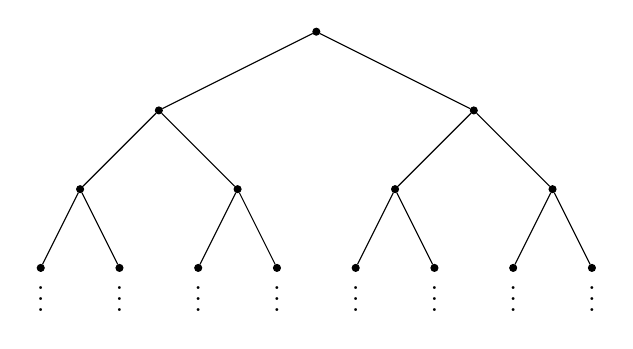
\begin{tikzpicture}
      \node[fill,draw,circle,inner sep=0pt,minimum size=0.25em] (r) at (0,0){};

      \node[fill,draw,circle,inner sep=0pt,minimum size=0.25em] (r0) at (-2,-1){};
      \node[fill,draw,circle,inner sep=0pt,minimum size=0.25em] (r1) at (2,-1){};

      \node[fill,draw,circle,inner sep=0pt,minimum size=0.25em] (r00) at (-3,-2){};
      \node[fill,draw,circle,inner sep=0pt,minimum size=0.25em] (r01) at (-1,-2){};
      \node[fill,draw,circle,inner sep=0pt,minimum size=0.25em] (r10) at (1,-2){};
      \node[fill,draw,circle,inner sep=0pt,minimum size=0.25em] (r11) at (3,-2){};

      \node[fill,draw,circle,inner sep=0pt,minimum size=0.25em] (r000) at (-3.5,-3){};
      \node[fill,draw,circle,inner sep=0pt,minimum size=0.25em] (r001) at (-2.5,-3){};
      \node[fill,draw,circle,inner sep=0pt,minimum size=0.25em] (r010) at (-0.5,-3){};
      \node[fill,draw,circle,inner sep=0pt,minimum size=0.25em] (r011) at (-1.5,-3){};

      \node[fill,draw,circle,inner sep=0pt,minimum size=0.25em] (r110) at (3.5,-3){};
      \node[fill,draw,circle,inner sep=0pt,minimum size=0.25em] (r111) at (2.5,-3){};
      \node[fill,draw,circle,inner sep=0pt,minimum size=0.25em] (r100) at (0.5,-3){};
      \node[fill,draw,circle,inner sep=0pt,minimum size=0.25em] (r101) at (1.5,-3){};

      \node [below=-1ex of r000] {$\vdots$};
      \node [below=-1ex of r001] {$\vdots$};
      \node [below=-1ex of r010] {$\vdots$};
      \node [below=-1ex of r011] {$\vdots$};
      \node [below=-1ex of r100] {$\vdots$};
      \node [below=-1ex of r101] {$\vdots$};
      \node [below=-1ex of r110] {$\vdots$};
      \node [below=-1ex of r111] {$\vdots$};

      \draw[](r) -- (r0);
      \draw[](r) -- (r1);

      \draw[](r0) -- (r00);
      \draw[](r0) -- (r01);
      \draw[](r1) -- (r10);
      \draw[](r1) -- (r11);

      \draw[](r00) -- (r000);
      \draw[](r00) -- (r001);
      \draw[](r01) -- (r010);
      \draw[](r01) -- (r011);

      \draw[](r10) -- (r100);
      \draw[](r10) -- (r101);
      \draw[](r11) -- (r110);
      \draw[](r11) -- (r111);
    \end{tikzpicture}
  \end{center}

  Notice that every automorphism $x \in \mathrm{Aut}(\mathcal T)$ preserves the root (and each level).

  Moreover, given such an automorphism, we can write \emph{$x = (x_0,x_1)\cdot s$} where
  \vspace{-0.7em}\begin{itemize}\setlength\itemsep{-0.7em}
    \item \emph{$x_0 \in \mathrm{Aut}(\mathcal T)$} is an automorphism of the \underline{left subtree};
    \item \emph{$x_1 \in \mathrm{Aut}(\mathcal T)$} is an automorphism of the \underline{right subtree}; and
    \item \emph{$s \in \mathrm{Sym}(2)$} is a permutation of the first-level subtrees.
  \end{itemize}

\end{frame}


%%%%%%%%%%%%%%%%%%%%%%%%%%%%%%%%%%%%%%%%%%%%%%%%%%%%%%%%%%%%%%%%%%%%%%%%%%
%%%%%%%%%%%%%%%%%%%%%%%%%%%%%%%%%%%%%%%%%%%%%%%%%%%%%%%%%%%%%%%%%%%%%%%%%%

\begin{frame}
	\frametitle{The first Grigorchuk group}

	% Let $\mathcal T$ be the infinite rooted tree with vertex set $\{0,1\}^*$.

	The Grigorchuk group $\Grig = \left\langle a,b,c,d\right\rangle$ is generated by the tree automorphisms:
	\begin{center}
		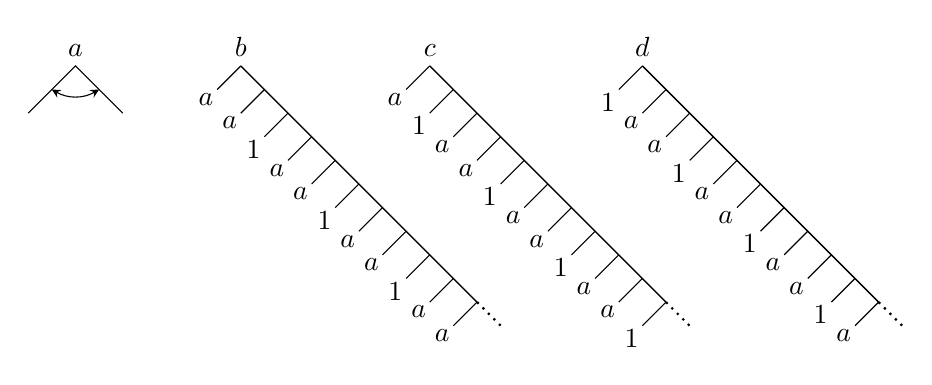
\begin{tikzpicture}[>=stealth,scale=0.3]

			\draw (0,0) -- (-2,2) node [above] {$a$} -- (-4,0);
			\draw [<->] (-3,1) to [bend right] (-1,1);

			\begin{scope}[shift={(7,0)}]
				\draw (0,0) -- (-2,2) node [above] {$b$} -- (8,-8);
				\foreach \x in {-2,-1,1,2,4,5,7,8} {
						\draw (\x,-\x) to +(-1,-1) node [below left=-0.3em] {$a$};
					}
				\foreach \x in {0,3,6} {
						\draw (\x,-\x) to +(-1,-1) node [below left=-0.3em] {$1$};
					}
				\draw [dotted,thick] (8,-8) to +(1,-1);
				\draw [] (-2,2) to (8,-8);
			\end{scope}

			\begin{scope}[shift={(15,0)}]
				\draw (0,0) -- (-2,2) node [above] {$c$} -- (8,-8);
				\foreach \x in {-2,0,1,3,4,6,7} {
						\draw (\x,-\x) to +(-1,-1) node [below left=-0.3em] {$a$};
					}
				\foreach \x in {-1,2,5,8} {
						\draw (\x,-\x) to +(-1,-1) node [below left=-0.3em] {$1$};
					}
				\draw [dotted,thick] (8,-8) to +(1,-1);
				\draw [] (-2,2) to (8,-8);
			\end{scope}

			\begin{scope}[shift={(24,0)}]
				\draw (0,0) -- (-2,2) node [above] {$d$} -- (8,-8);
				\foreach \x in {-1,0,2,3,5,6,8} {
						\draw (\x,-\x) to +(-1,-1) node [below left=-0.3em] {$a$};
					}
				\foreach \x in {-2,1,4,7} {
						\draw (\x,-\x) to +(-1,-1) node [below left=-0.3em] {$1$};
					}
				\draw [dotted,thick] (8,-8) to +(1,-1);
				\draw [] (-2,2) to (8,-8);
			\end{scope}
		\end{tikzpicture}
	\end{center}

	\begin{block}{Notation}
		We can write elements \emph{$g \in \Grig$} in the form \emph{$g = (g_0,g_1)\cdot s$} where \emph{$g_i\in \Grig$} is the action of the element on the $i$-th subtree, and \emph{$s \in \{1,\sigma\} =\mathrm{Sym}(2)$} is a permutation of the first level.

		For example, $a = (1,1)\cdot \sigma$, $b = (a,c)\cdot 1$, $c = (a,d)\cdot 1$ and $d = (1,b)\cdot 1$.
	\end{block}

\end{frame}

%%%%%%%%%%%%%%%%%%%%%%%%%%%%%%%%%%%%%%%%%%%%%%%%%%%%%%%%%%%%%%%%%%%%%%%%%%
%%%%%%%%%%%%%%%%%%%%%%%%%%%%%%%%%%%%%%%%%%%%%%%%%%%%%%%%%%%%%%%%%%%%%%%%%%

\begin{frame}[t]
	\frametitle{Stabiliser subgroups}

	For each $m\geq 1$, we define the \emph{stabiliser subgroup} $\mathrm{Stab}(m) \triangleleft \Grig$ as
	\[
		\mathrm{Stab}(m)
		=
		\{
		g\in \Grig
		\mid
		g(v) = v
		\text{ for each }
		v\in \{0,1\}^m
		\}.
	\]
	Each stabiliser subgroup is finite index in $\Grig$ with index given in the following lemma.

	\pause

	\begin{lemma}% (see p.~221 and Prop. 41 on p.~238 of ``Topics in geometric group theory''\nocite{harpe2000}).}
		\vspace{-1ex}
		\[
			[\Grig:\mathrm{Stab}(1)] = 2,\quad
			[\Grig:\mathrm{Stab}(2)] = 8\quad\text{and}\quad
			[\Grig:\mathrm{Stab}(m)] = 2^{5\cdot 2^{m-3}+2}
		\]
		for each $m \geq 3$.
	\end{lemma}

	\begin{block}{Example}
		\vspace{-1ex}
		\[
			\mathrm{Stab}(1)
			=
			\left\langle
			b,c,d,aba,aca,ada
			\right\rangle
			\qquad
			\text{where}
			\qquad
			\Grig = \{1,a\}\cdot \mathrm{Stab}(1)
		\]
	\end{block}

	\pause

	\begin{lemma}
		For each subgroup $N \triangleleft_{\mathrm{f.i.}} G$, there is an $m \geq 0$ such that
		\[
			\mathrm{Stab}(m+5)
			\leq
			N
			\leq
			\mathrm{Stab}(m).
		\]
		Thus, the size of $G/N$ can be bound between the sizes of quotients by stabiliser subgroups.
	\end{lemma}
\end{frame}

%%%%%%%%%%%%%%%%%%%%%%%%%%%%%%%%%%%%%%%%%%%%%%%%%%%%%%%%%%%%%%%%%%%%%%%%%%
%%%%%%%%%%%%%%%%%%%%%%%%%%%%%%%%%%%%%%%%%%%%%%%%%%%%%%%%%%%%%%%%%%%%%%%%%%

\begin{frame}
	\frametitle{Our result}
	\begin{theorem}
		The conjugacy depth function for the Grigorchuk group, $\Grig$, is bounded as
			{\large\[
					e^n
					\preccurlyeq
					\Conj_\Grig(n)
					\preccurlyeq
					e^{n^{\alpha}}
				\]}
		where $\alpha = 2.7350028...\,.$
	\end{theorem}

	\pause

	\bigskip

	\textit{Proof idea.}
	\begin{itemize}
		\item The lower bound of $e^n$ comes from a result of {\color{OwlGreen}\textcite{BR2010}}, who showed that the \emph{residual finiteness depth} (which is a lower bound for conjugacy depth) is $e^n$.
		\item  For the upper bound, we consider a recursive algorithm for the conjugacy problem.
	\end{itemize}

	% \bigskip
	%
	%
	%
	%
	% \question{Which quotients of the Grigorchuk group are used in this proof?}

\end{frame}

%%%%%%%%%%%%%%%%%%%%%%%%%%%%%%%%%%%%%%%%%%%%%%%%%%%%%%%%%%%%%%%%%%%%%%%%%%
%%%%%%%%%%%%%%%%%%%%%%%%%%%%%%%%%%%%%%%%%%%%%%%%%%%%%%%%%%%%%%%%%%%%%%%%%%

\section{From the Literature:\\An algorithm for the conjugacy problem in Grigorchuk group}

\begin{frame}[t]
	\frametitle{The branch subgroup}

	Let $\SubK = \left\langle (ab)^2 \right\rangle^\Grig$ be the normal closure of $(ab)^2$ in $\Grig$, that is,
	\[
		\SubK
		=
		\left\langle
		(ab)^2,
		(bada)^2,
		(abad)^2
		\right\rangle.
	\]
	Then, we note here that $\SubK$ is finite index in $\Grig$, in particular, $[\Grig:\SubK]=16$.

	\begin{definition}
		We define the function $Q\colon \Grig\times\Grig\to \PowerSet{\Grig/\SubK}$ as
		\[
			Q(g,h)
			=
			\{
			\SubK x
			\mid
			g = xhx^{-1}
			\text{ where }
			x\in \Grig
			\}.
		\]
		We then see that $Q(g,h)=\emptyset$ if and only if $g\not\sim_\Grig h$.
	\end{definition}

	\begin{block}{Example}
		\begin{align*}
			Q(a,a) & = \SubK\{1,a,dad,(ad)^2\},                 &
			Q(b,b) & = \SubK\{1,b,c,d\},                          \\
			Q(c,c) & = \SubK\{1,b,c,d\}\ \ \text{and}           &
			Q(d,d) & = \SubK\{1,b,c,d,ada,(ad)^2,bada, badad\}.
		\end{align*}
		Moreover, $Q(1,1)=\Grig/\SubK$; and if $x,y\in \{a,b,c,d,1\}$ with $x\neq y$, then $Q(x,y)=\emptyset$.
	\end{block}

	% \question{We may then compute the value of $Q(g,h)$ recursively using the fomulas on the next slide.}
\end{frame}

%%%%%%%%%%%%%%%%%%%%%%%%%%%%%%%%%%%%%%%%%%%%%%%%%%%%%%%%%%%%%%%%%%%%%%%%%%
%%%%%%%%%%%%%%%%%%%%%%%%%%%%%%%%%%%%%%%%%%%%%%%%%%%%%%%%%%%%%%%%%%%%%%%%%%

\begin{frame}
	\frametitle{Why the subgroup $\SubK$}

	\begin{definition}
		From the subgroup $K$, we may define a map
		$\mathrm{Lift}\colon \PowerSet{\Grig/\SubK \times \Grig/\SubK}\to \PowerSet{\Grig/\SubK}$
		as
		\[
			\mathrm{Lift}(S)
			\coloneq
			\{
			Kg \mid
			\text{where }g=(g_0,g_1)\cdot 1\in\mathrm{Stab}(1)
			\text{ with }(Kg_0,Kg_1)\in S
			\}.
		\]
		This map has the following property.
	\end{definition}

	Suppose that $g_0,g_1\in \Gamma$.

	Then there is an element $g\in \mathrm{Stab}(1)\subset \Gamma$
	such that $g = (g_0,g_1)\cdot 1$ if and only if
	\[
		\mathrm{Lift}(\{(Kg_0,Kg_1)\}) \neq \emptyset.
	\]
	Moreover, for each
	\[
		Kh \in
		\mathrm{Lift}(\{(Kg_0,Kg_1)\}),
	\]
	there exists such a $g$ with $Kg = Kh$.
	% Let $\SubK = \left\langle (ab)^2 \right\rangle^\Grig$ be the normal closure of $(ab)^2$ in $\Grig$, that is,
	% \[
	% 	\SubK
	% 	=
	% 	\left\langle
	% 	(ab)^2,
	% 	(bada)^2,
	% 	(abad)^2
	% 	\right\rangle.
	% \]
	% Then, we note here that $\SubK$ is finite index in $\Grig$, in particular, $[\Grig:\SubK]=16$.
	%
	% \begin{definition}
	% 	We define the function $Q\colon \Grig\times\Grig\to \PowerSet{\Grig/\SubK}$ as
	% 	\[
	% 		Q(g,h)
	% 		=
	% 		\{
	% 		\SubK x
	% 		\mid
	% 		g = xhx^{-1}
	% 		\text{ where }
	% 		x\in \Grig
	% 		\}.
	% 	\]
	% 	We then see that $Q(g,h)=\emptyset$ if and only if $g\not\sim_\Grig h$.
	% \end{definition}
	%
	% \begin{lemma}
	% 	\justifying
	% 	There exists a function $\mathrm{Lift}\colon \PowerSet{\Grig/\SubK \times \Grig/\SubK}\to \PowerSet{\Grig/\SubK}$ with the following property.
	%
	% 	Suppose that $g_0,g_1\in \Grig$ with $k_0=\SubK g_0$ and $k_1=\SubK g_1$.
	% 	Then, there is some $g = (g_0,g_1)\cdot 1\in \Grig$ if and only if $\mathrm{Lift}(\{(k_0,k_1)\}) \neq \emptyset$.
	% 	In particular, we would have that $\SubK g \in \mathrm{Lift}(\{(k_0,k_1)\})$.
	% \end{lemma}

\end{frame}

%%%%%%%%%%%%%%%%%%%%%%%%%%%%%%%%%%%%%%%%%%%%%%%%%%%%%%%%%%%%%%%%%%%%%%%%%%
%%%%%%%%%%%%%%%%%%%%%%%%%%%%%%%%%%%%%%%%%%%%%%%%%%%%%%%%%%%%%%%%%%%%%%%%%%

\begin{frame}
	\frametitle{Recursively computing $Q(g,h)$}

	We may then compute the value of $Q(g,h)$ recursively as follows.

	\begin{lemma}
		\begin{enumerate}
			\item if $g = (g_0,g_1)\cdot 1\in \mathrm{Stab}(1)$ and $h = (h_0,h_1)\cdot 1\in \mathrm{Stab}(1)$, then
			      \[
				      Q(g,h)
				      =
				      \mathrm{Lift}\left(
				      \focus{Q(g_0, h_0)}
				      \times
				      \focus{Q(g_1, h_1)} \right)
				      \cup
				      \mathrm{Lift}\left( \focus{Q(g_1,h_0)} \times \focus{Q(g_0, h_1)} \right);
			      \]
			\item if $g=(g_0,g_1)\cdot \sigma\notin \mathrm{Stab}(1)$ and $h=(g_0,g_1)\cdot \sigma\notin \mathrm{Stab}(1)$, then
			      \begin{multline*}
				      Q(g,h)
				      =
				      \mathrm{Lift}\left\{
				      (\SubK \,x_0, \SubK\, x_1)
				      \ \middle|\
				      \begin{aligned}
					      \SubK\, x_0 \in \focus{Q(g_0 g_1, h_0 h_1)}
					      \\\text{ and }
					      \SubK\, x_1 = \SubK\, h_1 x_0 g_1^{-1}
				      \end{aligned}
				      \right\}
				      \\\cup
				      \mathrm{Lift}\left\{
				      (\SubK\, x_0, \SubK\, x_1)
				      \ \middle|\
				      \begin{aligned}
					      \SubK\, x_0 \in \focus{Q(g_1 g_0, h_0 h_1)}
					      \\\text{ and }
					      \SubK\, x_1 = \SubK\, h_1 x_0 g_0^{-1}
				      \end{aligned}
				      \right\};
			      \end{multline*}
			\item in all remaining cases $Q(g,h) = \emptyset.$
		\end{enumerate}
	\end{lemma}%
\end{frame}

%%%%%%%%%%%%%%%%%%%%%%%%%%%%%%%%%%%%%%%%%%%%%%%%%%%%%%%%%%%%%%%%%%%%%%%%%%
%%%%%%%%%%%%%%%%%%%%%%%%%%%%%%%%%%%%%%%%%%%%%%%%%%%%%%%%%%%%%%%%%%%%%%%%%%

\begin{frame}
	\frametitle{Algorithm recursion cases}

	Thus, we can construct a tree which locally looks like one of the following pictures.

	\begin{center}
		\begin{minipage}[t]{0.45\linewidth}
			\begin{framed}
				\centering
				If $g,h\in \mathrm{Stab}(1)$, then

				\medskip

				\resizebox{\linewidth}{!}{
					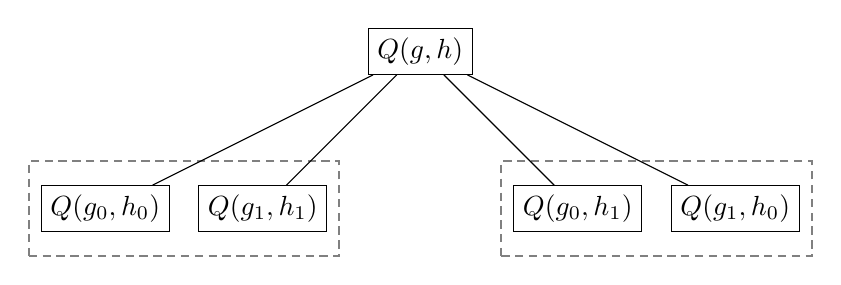
\begin{tikzpicture}[>=stealth]
						\node[draw] (n) at (0,0) {$Q(g,h)$};

						\node[draw] (nl0) at (-4,-2) {$Q(g_0, h_0)$};
						\node[draw] (nl1) at (-2,-2) {$Q(g_1, h_1)$};

						\node[draw] (nr0) at (4,-2) {$Q(g_1, h_0)$};
						\node[draw] (nr1) at (2,-2) {$Q(g_0, h_1)$};

						\node[draw=gray, thick,
							densely dashed,
							inner xsep=1ex, inner ysep=2ex,
							fit=(nl0) (nl1)] {};
						\node[draw=gray, thick,
							densely dashed,
							inner xsep=1ex, inner ysep=2ex,
							fit=(nr0) (nr1)] {};

						\draw[] (nl0) to (n);
						\draw[] (nl1) to (n);
						\draw[] (nr0) to (n);
						\draw[] (nr1) to (n);

					\end{tikzpicture}}
			\end{framed}
		\end{minipage}
		\begin{minipage}[t]{0.45\linewidth}
			\begin{framed}
				\centering
				If $g,h\notin \mathrm{Stab}(1)$, then

				\medskip

				\resizebox{\linewidth}{!}{
					\begin{tikzpicture}[>=stealth]
						\node[draw] (n) at (0,0) {$Q(g,h)$};

						\node[draw] (nl0) at (-3,-2) {$Q(g_0g_1, h_0h_1)$};

						\node[draw] (nr0) at (3,-2) {$Q(g_1g_0, h_0h_1)$};

						\draw[]  (nl0) to (n);
						\draw[]  (nr0) to (n);

						\phantom{
							\node[draw] (n) at (0,0) {$Q(g,h)$};
							\node[draw] (nl0) at (-4,-2) {$Q(g_0, h_0)$};
							\node[draw] (nr0) at (4,-2) {$Q(g_1, h_0)$};
							\node[draw] (nr1) at (2,-2) {$Q(g_0, h_1)$};
							\node[draw=gray, thick,
								densely dashed,
								inner xsep=1ex, inner ysep=2ex,
								fit=(nl0) (nl1)] {};
							\node[draw=gray, thick,
								densely dashed,
								inner xsep=1ex, inner ysep=2ex,
								fit=(nr0) (nr1)] {};
							\draw[] (nl0) to (n);
							\draw[] (nl1) to (n);
							\draw[] (nr0) to (n);
							\draw[] (nr1) to (n);
						}
					\end{tikzpicture}}
			\end{framed}
		\end{minipage}
	\end{center}

	%   \pause
	%
	%   \bigskip
	%
	%   For each pair of elements, $g,h\in \Grig$, we can then describe a finite graph,
	%   \begin{itemize}
	%     \item the root is labelled by $Q(g,h)$; and
	%     \item the leaves have labels of the form $Q(x,y)$ with $x,y\in \{a,b,c,d,1\}$.
	% \end{itemize}
\end{frame}

%%%%%%%%%%%%%%%%%%%%%%%%%%%%%%%%%%%%%%%%%%%%%%%%%%%%%%%%%%%%%%%%%%%%%%%%%%
%%%%%%%%%%%%%%%%%%%%%%%%%%%%%%%%%%%%%%%%%%%%%%%%%%%%%%%%%%%%%%%%%%%%%%%%%%

\begin{frame}
	\frametitle{Splitting tree}

	\bigskip

	\begin{center}
		\scalebox{0.7}{
			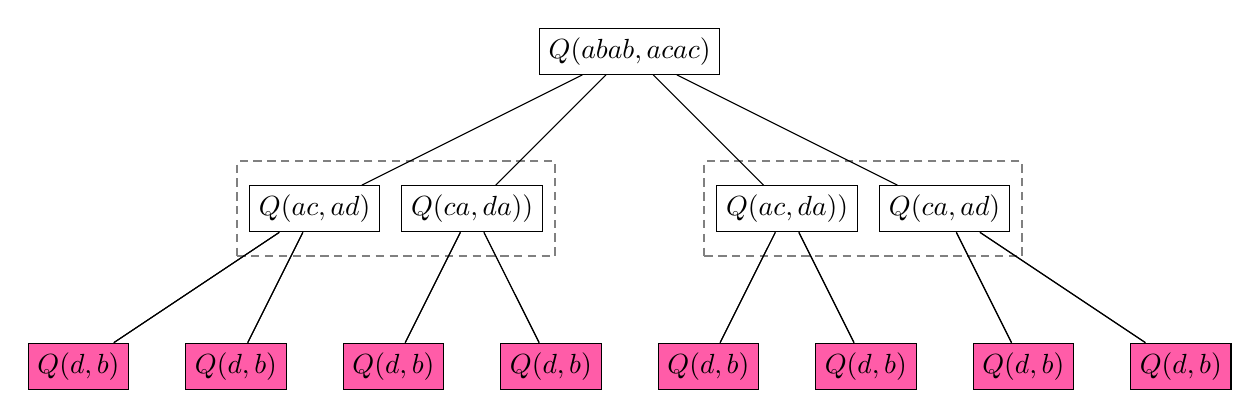
\begin{tikzpicture}[>=stealth]

				\node[draw] (n) at (0,0) {$Q(abab, acac)$};

				% LEVEL 1

				\visible<2->{
					\node[draw] (nl0) at (-4,-2) {$Q(ac,ad)$};
					\node[draw] (nl1) at (-2,-2) {$Q(ca,da))$};
					\node[draw=gray, thick, densely dashed, inner xsep=1ex, inner ysep=2ex, fit=(nl0) (nl1)] {};

					\node[draw] (nr1) at (2,-2) {$Q(ac,da))$};
					\node[draw] (nr0) at (4,-2) {$Q(ca,ad)$};
					\node[draw=gray, thick, densely dashed, inner xsep=1ex, inner ysep=2ex, fit=(nr0) (nr1)] {};

					\draw[] (nl0) to (n);
					\draw[] (nl1) to (n);
					\draw[] (nr0) to (n);
					\draw[] (nr1) to (n);
				}
				% LEVEL 2

				\visible<3>{
					\node[draw] (nl0l) at (-7,-4) {$Q(d,b)$};
					\node[draw] (nl0r) at (-5,-4) {$Q(d,b)$};

					\node[draw] (nl1l) at (-3,-4) {$Q(d,b)$};
					\node[draw] (nl1r) at (-1,-4) {$Q(d,b)$};

					\node[draw] (nr0l) at (1,-4) {$Q(d,b)$};
					\node[draw] (nr0r) at (3,-4) {$Q(d,b)$};

					\node[draw] (nr1l) at (5,-4) {$Q(d,b)$};
					\node[draw] (nr1r) at (7,-4) {$Q(d,b)$};

					\draw[] (nl0l) to (nl0);
					\draw[] (nl0r) to (nl0);
					\draw[] (nl1l) to (nl1);
					\draw[] (nl1r) to (nl1);

					\draw[] (nr0l) to (nr1);
					\draw[] (nr0r) to (nr1);
					\draw[] (nr1l) to (nr0);
					\draw[] (nr1r) to (nr0);
				}
				\visible<4->{
					\node[draw,fill=RedAlert] (nl0l) at (-7,-4) {$Q(d,b)$};
					\node[draw,fill=RedAlert] (nl0r) at (-5,-4) {$Q(d,b)$};

					\node[draw,fill=RedAlert] (nl1l) at (-3,-4) {$Q(d,b)$};
					\node[draw,fill=RedAlert] (nl1r) at (-1,-4) {$Q(d,b)$};

					\node[draw,fill=RedAlert] (nr0l) at (1,-4) {$Q(d,b)$};
					\node[draw,fill=RedAlert] (nr0r) at (3,-4) {$Q(d,b)$};

					\node[draw,fill=RedAlert] (nr1l) at (5,-4) {$Q(d,b)$};
					\node[draw,fill=RedAlert] (nr1r) at (7,-4) {$Q(d,b)$};

					\draw[] (nl0l) to (nl0);
					\draw[] (nl0r) to (nl0);
					\draw[] (nl1l) to (nl1);
					\draw[] (nl1r) to (nl1);

					\draw[] (nr0l) to (nr1);
					\draw[] (nr0r) to (nr1);
					\draw[] (nr1l) to (nr0);
					\draw[] (nr1r) to (nr0);
				}
			\end{tikzpicture}}
	\end{center}


	\bigskip
	\visible<4>{
		\begin{block}{Recall}
			\begin{align*}
				Q(a,a) & = \SubK\{1,a,dad,(ad)^2\},                 &
				Q(b,b) & = \SubK\{1,b,c,d\},                          \\
				Q(c,c) & = \SubK\{1,b,c,d\}\ \ \text{and}           &
				Q(d,d) & = \SubK\{1,b,c,d,ada,(ad)^2,bada, badad\}.
			\end{align*}
			Moreover, $Q(1,1)=\Grig/\SubK$; and {\color{OwlYellow}if $x,y\in \{a,b,c,d,1\}$ with $x\neq y$, then $Q(x,y)=\emptyset$}.
		\end{block}

		\textbf{Conclusion:} We then see that, \emph{$abab \not\sim_\Grig acac$}.
	}
\end{frame}

\section{Our Proof Method:\\A finite quotients version}

%%%%%%%%%%%%%%%%%%%%%%%%%%%%%%%%%%%%%%%%%%%%%%%%%%%%%%%%%%%%%%%%%%%%%%%%%%
%%%%%%%%%%%%%%%%%%%%%%%%%%%%%%%%%%%%%%%%%%%%%%%%%%%%%%%%%%%%%%%%%%%%%%%%%%
\begin{frame}[t]
	\frametitle{Finite quotient version: map $Q$}

	~

	\begin{definition}
		We define the function $Q\colon \Grig\times\Grig\to \PowerSet{\Grig/\SubK}$ as
		\[
			Q(g,h)
			=
			\{
			\SubK x
			\mid
			g = xhx^{-1}
			\text{ where }
			x\in \Grig
			\}.
		\]
		We then see that $Q(g,h)=\emptyset$ if and only if $g\not\sim_\Grig h$.


		\visible<2->{
			For each $m \geq 3$, we define the function $Q_{{\color{OwlYellow}m}}\colon ({\color{OwlYellow}\Grig/\mathrm{Stab}(m)})^2\to \PowerSet{\Grig/\SubK}$ as
			\[
				Q_{{\color{OwlYellow}m}}(g,h)
				=
				\{
				\SubK x
				\mid
				g = xhx^{-1}
				\text{ within }{\color{OwlYellow}\Grig/\mathrm{Stab}(m)}
				\text{ where }
				x\in {\color{OwlYellow}\Grig/\mathrm{Stab}(m)}
				\}.
			\]
			We then see that $Q_{{\color{OwlYellow}m}}(g,h)=\emptyset$ if and only if $g\not\sim_{{\color{OwlYellow}\Grig/\mathrm{Stab}(m)}} h$.
		}
	\end{definition}
	\only<3->{
		\begin{lemma}
			For each ${\color{OwlYellow}m \geq 4}$, we have ${\color{OwlYellow}Q_m(x,y) = Q(x,y)}$ for each ${\color{OwlYellow}x,y\in \{a,b,c,d,1\}}$.\footnote{Note that $m\geq 4$ is needed here, in particular, $Q(c,c)\neq Q_3(c,c)$.}
		\end{lemma}}
\end{frame}

%%%%%%%%%%%%%%%%%%%%%%%%%%%%%%%%%%%%%%%%%%%%%%%%%%%%%%%%%%%%%%%%%%%%%%%%%%
%%%%%%%%%%%%%%%%%%%%%%%%%%%%%%%%%%%%%%%%%%%%%%%%%%%%%%%%%%%%%%%%%%%%%%%%%%
\begin{frame}
	\frametitle{Finite quotient version: example tree}

	\begin{center}
		\scalebox{0.7}{
			\begin{tikzpicture}[>=stealth]

				\node[draw] (n) at (0,0) {$Q(abab, acac)$};

				% LEVEL 1

				\node[draw] (nl0) at (-4,-2) {$Q(ac,ad)$};
				\node[draw] (nl1) at (-2,-2) {$Q(ca,da))$};
				\node[draw=gray, thick, densely dashed, inner xsep=1ex, inner ysep=2ex, fit=(nl0) (nl1)] {};

				\node[draw] (nr1) at (2,-2) {$Q(ac,da))$};
				\node[draw] (nr0) at (4,-2) {$Q(ca,ad)$};
				\node[draw=gray, thick, densely dashed, inner xsep=1ex, inner ysep=2ex, fit=(nr0) (nr1)] {};

				\draw[] (nl0) to (n);
				\draw[] (nl1) to (n);
				\draw[] (nr0) to (n);
				\draw[] (nr1) to (n);
				% LEVEL 2

				\only<1>{
					\node[draw] (nl0l) at (-7,-4) {$Q(d,b)$};
					\node[draw] (nl0r) at (-5,-4) {$Q(d,b)$};

					\node[draw] (nl1l) at (-3,-4) {$Q(d,b)$};
					\node[draw] (nl1r) at (-1,-4) {$Q(d,b)$};

					\node[draw] (nr0l) at (1,-4) {$Q(d,b)$};
					\node[draw] (nr0r) at (3,-4) {$Q(d,b)$};

					\node[draw] (nr1l) at (5,-4) {$Q(d,b)$};
					\node[draw] (nr1r) at (7,-4) {$Q(d,b)$};
				}
				\only<2->{
					\node[draw,fill=OwlRed] (nl0l) at (-7,-4) {$Q_{4}(d,b)$};
					\node[draw,fill=OwlRed] (nl0r) at (-5,-4) {$Q_4(d,b)$};

					\node[draw,fill=OwlRed] (nl1l) at (-3,-4) {$Q_4(d,b)$};
					\node[draw,fill=OwlRed] (nl1r) at (-1,-4) {$Q_4(d,b)$};

					\node[draw,fill=OwlRed] (nr0l) at (1,-4) {$Q_4(d,b)$};
					\node[draw,fill=OwlRed] (nr0r) at (3,-4) {$Q_4(d,b)$};

					\node[draw,fill=OwlRed] (nr1l) at (5,-4) {$Q_4(d,b)$};
					\node[draw,fill=OwlRed] (nr1r) at (7,-4) {$Q_4(d,b)$};
				}
				\draw[] (nl0l) to (nl0);
				\draw[] (nl0r) to (nl0);
				\draw[] (nl1l) to (nl1);
				\draw[] (nl1r) to (nl1);

				\draw[] (nr0l) to (nr1);
				\draw[] (nr0r) to (nr1);
				\draw[] (nr1l) to (nr0);
				\draw[] (nr1r) to (nr0);
			\end{tikzpicture}}
	\end{center}
\end{frame}

%%%%%%%%%%%%%%%%%%%%%%%%%%%%%%%%%%%%%%%%%%%%%%%%%%%%%%%%%%%%%%%%%%%%%%%%%%
%%%%%%%%%%%%%%%%%%%%%%%%%%%%%%%%%%%%%%%%%%%%%%%%%%%%%%%%%%%%%%%%%%%%%%%%%%

\begin{frame}
	\frametitle{Finite quotient version: recursive definition}
	\begin{lemma}
		\visible<2->{For all {\color{OwlYellow}$m \geq 3$}:}
		\begin{enumerate}
			\item if $g = (g_0,g_1)\cdot 1\in \mathrm{Stab}(1)$ and $h = (h_0,h_1)\cdot 1\in \mathrm{Stab}(1)$, then
			      \[
				      Q_{\only<2->{{\color{OwlYellow}m+1}}}(g,h)
				      =
				      \mathrm{Lift}\left(
				      {Q_{\only<2->{{\color{OwlYellow}m}}}(g_0, h_0)}
				      \times
					      {Q_{\only<2->{{\color{OwlYellow}m}}}(g_1, h_1)} \right)
				      \cup
				      \mathrm{Lift}\left( {Q_{\only<2->{{\color{OwlYellow}m}}}(g_1,h_0)} \times {Q_{\only<2->{{\color{OwlYellow}m}}}(g_0, h_1)} \right);
			      \]
			\item if $g=(g_0,g_1)\cdot \sigma\notin\mathrm{Stab}(1)$ and $h=(g_0,g_1)\cdot \sigma\notin \mathrm{Stab}(1)$, then
			      \begin{multline*}
				      Q_{\only<2->{{\color{OwlYellow}m+1}}}(g,h)
				      =
				      \mathrm{Lift}\left\{
				      (\SubK \,x_0, \SubK\, x_1)
				      \ \middle|\
				      \begin{aligned}
					      \SubK\, x_0 \in {Q_{\only<2->{{\color{OwlYellow}m}}}(g_0 g_1, h_0 h_1)}
					      \\\text{ and }
					      \SubK\, x_1 = \SubK\, h_1 x_0 g_1^{-1}
				      \end{aligned}
				      \right\}
				      \\\cup
				      \mathrm{Lift}\left\{
				      (\SubK\, x_0, \SubK\, x_1)
				      \ \middle|\
				      \begin{aligned}
					      \SubK\, x_0 \in {Q_{\only<2->{{\color{OwlYellow}m}}}(g_1 g_0, h_0 h_1)}
					      \\\text{ and }
					      \SubK\, x_1 = \SubK\, h_1 x_0 g_0^{-1}
				      \end{aligned}
				      \right\};
			      \end{multline*}
			\item in all remaining cases $Q_{\only<2->{{\color{OwlYellow}m+1}}}(g,h) = \emptyset.$
		\end{enumerate}
	\end{lemma}%
\end{frame}
%%%%%%%%%%%%%%%%%%%%%%%%%%%%%%%%%%%%%%%%%%%%%%%%%%%%%%%%%%%%%%%%%%%%%%%%%%
%%%%%%%%%%%%%%%%%%%%%%%%%%%%%%%%%%%%%%%%%%%%%%%%%%%%%%%%%%%%%%%%%%%%%%%%%%

%%%%%%%%%%%%%%%%%%%%%%%%%%%%%%%%%%%%%%%%%%%%%%%%%%%%%%%%%%%%%%%%%%%%%%%%%%
%%%%%%%%%%%%%%%%%%%%%%%%%%%%%%%%%%%%%%%%%%%%%%%%%%%%%%%%%%%%%%%%%%%%%%%%%%
\begin{frame}[t]
	\frametitle{Finite quotient version: example tree (part 2)}

	\begin{center}
		\scalebox{0.7}{
			\begin{tikzpicture}[>=stealth]

				\only<-2>{
					\node[draw] (n) at (0,0) {$Q(abab, acac)$};
				}
				\only<3-> {
					\node[draw,fill=OwlRed] (n) at (0,0) {$Q_6(abab, acac)$};
				}

				% LEVEL 1

				\only<1>{
					\node[draw] (nl0) at (-4,-2) {$Q(ac,ad)$};
					\node[draw] (nl1) at (-2,-2) {$Q(ca,da))$};
					\node[draw=gray, thick, densely dashed, inner xsep=1ex, inner ysep=2ex, fit=(nl0) (nl1)] {};
				}
				\only<2->{
					\node[draw,fill=OwlRed] (nl0) at (-4,-2) {$Q_5(ac,ad)$};
					\node[draw,fill=OwlRed] (nl1) at (-2,-2) {$Q_5(ca,da))$};
					\node[draw=gray, thick, densely dashed, inner xsep=1ex, inner ysep=2ex, fit=(nl0) (nl1)] {};
				}

				\only<1>{
					\node[draw] (nr1) at (2,-2) {$Q(ac,da))$};
					\node[draw] (nr0) at (4,-2) {$Q(ca,ad)$};
					\node[draw=gray, thick, densely dashed, inner xsep=1ex, inner ysep=2ex, fit=(nr0) (nr1)] {};
				}
				\only<2->{
					\node[draw,fill=OwlRed] (nr1) at (2,-2) {$Q_5(ac,da))$};
					\node[draw,fill=OwlRed] (nr0) at (4,-2) {$Q_5(ca,ad)$};
					\node[draw=gray, thick, densely dashed, inner xsep=1ex, inner ysep=2ex, fit=(nr0) (nr1)] {};
				}

				\draw[] (nl0) to (n);
				\draw[] (nl1) to (n);
				\draw[] (nr0) to (n);
				\draw[] (nr1) to (n);
				% LEVEL 2

				\node[draw,fill=OwlRed] (nl0l) at (-7,-4) {$Q_{4}(d,b)$};
				\node[draw,fill=OwlRed] (nl0r) at (-5,-4) {$Q_4(d,b)$};

				\node[draw,fill=OwlRed] (nl1l) at (-3,-4) {$Q_4(d,b)$};
				\node[draw,fill=OwlRed] (nl1r) at (-1,-4) {$Q_4(d,b)$};

				\node[draw,fill=OwlRed] (nr0l) at (1,-4) {$Q_4(d,b)$};
				\node[draw,fill=OwlRed] (nr0r) at (3,-4) {$Q_4(d,b)$};

				\node[draw,fill=OwlRed] (nr1l) at (5,-4) {$Q_4(d,b)$};
				\node[draw,fill=OwlRed] (nr1r) at (7,-4) {$Q_4(d,b)$};

				\draw[] (nl0l) to (nl0);
				\draw[] (nl0r) to (nl0);
				\draw[] (nl1l) to (nl1);
				\draw[] (nl1r) to (nl1);

				\draw[] (nr0l) to (nr1);
				\draw[] (nr0r) to (nr1);
				\draw[] (nr1l) to (nr0);
				\draw[] (nr1r) to (nr0);
			\end{tikzpicture}}
	\end{center}

	\bigskip

	\visible<3->{
		Thus, $Q_6(abab, acac)=\emptyset$ and hence $abab$ and $acac$ are not conjugate in $\Grig/\mathrm{Stab}(6)$.

		This then implies that $\ConjE_\Gamma(abab,acac)\leq |\Grig/\mathrm{Stab}(6)|$.

		\medskip

		\begin{lemma}
			If the tree for $Q(g,h)$ has depth $m$, then $\ConjE_\Gamma(g,h) \leq |\Grig/\mathrm{Stab}(m+4)|$.
		\end{lemma}
	}
\end{frame}

%%%%%%%%%%%%%%%%%%%%%%%%%%%%%%%%%%%%%%%%%%%%%%%%%%%%%%%%%%%%%%%%%%%%%%%%%%
%%%%%%%%%%%%%%%%%%%%%%%%%%%%%%%%%%%%%%%%%%%%%%%%%%%%%%%%%%%%%%%%%%%%%%%%%%

\begin{frame}[t]
	\frametitle{Tree Depth}

	\begin{center}
		\scalebox{0.7}{
			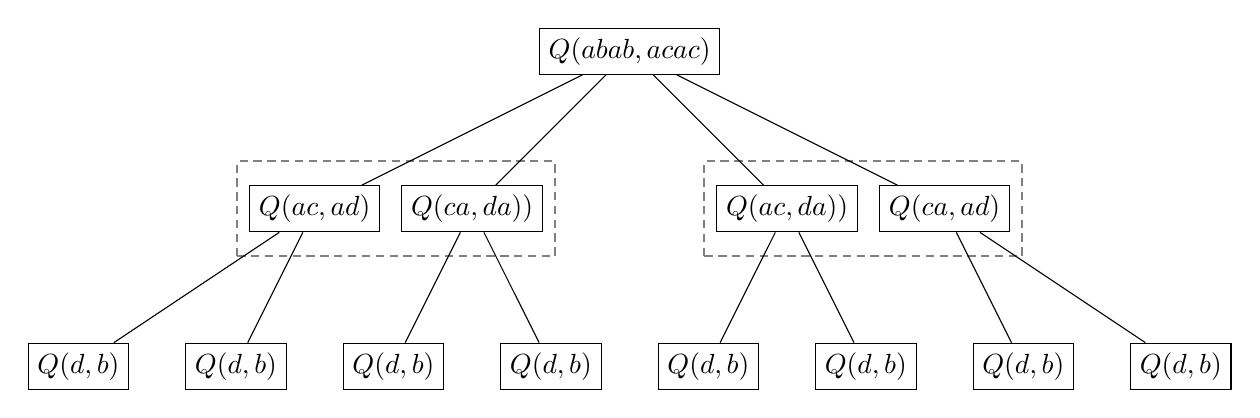
\begin{tikzpicture}[>=stealth]

				\node[draw] (n) at (0,0) {$Q(abab, acac)$};

				% LEVEL 1

				\node[draw] (nl0) at (-4,-2) {$Q(ac,ad)$};
				\node[draw] (nl1) at (-2,-2) {$Q(ca,da))$};
				\node[draw=gray, thick, densely dashed, inner xsep=1ex, inner ysep=2ex, fit=(nl0) (nl1)] {};
				\node[draw] (nr1) at (2,-2) {$Q(ac,da))$};
				\node[draw] (nr0) at (4,-2) {$Q(ca,ad)$};
				\node[draw=gray, thick, densely dashed, inner xsep=1ex, inner ysep=2ex, fit=(nr0) (nr1)] {};

				\draw[] (nl0) to (n);
				\draw[] (nl1) to (n);
				\draw[] (nr0) to (n);
				\draw[] (nr1) to (n);
				% LEVEL 2

				\node[draw] (nl0l) at (-7,-4) {$Q(d,b)$};
				\node[draw] (nl0r) at (-5,-4) {$Q(d,b)$};

				\node[draw] (nl1l) at (-3,-4) {$Q(d,b)$};
				\node[draw] (nl1r) at (-1,-4) {$Q(d,b)$};

				\node[draw] (nr0l) at (1,-4) {$Q(d,b)$};
				\node[draw] (nr0r) at (3,-4) {$Q(d,b)$};

				\node[draw] (nr1l) at (5,-4) {$Q(d,b)$};
				\node[draw] (nr1r) at (7,-4) {$Q(d,b)$};

				\draw[] (nl0l) to (nl0);
				\draw[] (nl0r) to (nl0);
				\draw[] (nl1l) to (nl1);
				\draw[] (nl1r) to (nl1);

				\draw[] (nr0l) to (nr1);
				\draw[] (nr0r) to (nr1);
				\draw[] (nr1l) to (nr0);
				\draw[] (nr1r) to (nr0);
			\end{tikzpicture}}
	\end{center}

	\bigskip

	\begin{lemma}
		If the tree for $Q(g,h)$ has depth $m$, then $\ConjE_\Grig(g,h) \leq |\Grig/\mathrm{Stab}(m+4)|$.
	\end{lemma}

	\begin{definition}
		The \emph{size} of a node $Q(g,h)$ in the above diagram is given by $\max\{\ell_\delta(g),\ell_\delta(h)\}$.
	\end{definition}

	\textbf{Idea:} We show that the size of a node's subtrees is \underline{fraction} of its size.

\end{frame}


%%%%%%%%%%%%%%%%%%%%%%%%%%%%%%%%%%%%%%%%%%%%%%%%%%%%%%%%%%%%%%%%%%%%%%%%%%
%%%%%%%%%%%%%%%%%%%%%%%%%%%%%%%%%%%%%%%%%%%%%%%%%%%%%%%%%%%%%%%%%%%%%%%%%%

\begin{frame}
	\frametitle{Bartholdi's weights}

	Let \emph{$\eta=0.8105357...$} be the real root of $x^3+x^2+x-2$, we define $\delta \colon X \to \mathbb R$ as
	\[
		\begin{aligned}
			\delta(a) & = 1-\eta^3 = 0.46750...,    &
			\delta(b) & = \eta^3   = 0.53249...,
			\\
			\delta(c) & = 1-\eta^2 = 0.34303...,    &
			\delta(d) & = 1-\eta   = 0.189464...\,.
		\end{aligned}
	\]
	Recall that we then define the weighted length as
	\[
		\ell_\delta(g)
		=
		\min\{
		\delta(w_1)+\delta(w_2)+\cdots+ \delta(w_k)
		\mid
		w=w_1 w_2 \cdots w_k\in X^*
		\text{ with }
		\overline{w}=g
		\}.
	\]

	\begin{lemma}[{{\color{OwlGreen}\cite{Bartholdi1998}}}]
		For each $g=(g_0,g_1)\cdot s\in \Grig$, we have
		\emph{$
				\ell_\delta(g_0) + \ell_\delta(g_1)
				\leq
				\eta\cdot
				(
				\ell_\delta(g)
				+\delta(a)
				)
			$}.
	\end{lemma}

	\pause
	\begin{lemma}
		There are constants $\varepsilon>0$ and $C\geq 0$ such that for each $g\in \Grig$, we have
		\emph{\[
				\ell_\delta(g_0), \ell_\delta(g_1)
				\leq
				\mu\cdot(\ell_\delta(g)+C)
			\]}
		where
		\emph{\[
				\mu =
				\frac{\ell_\delta(ab)}{\ell_\delta(cada)}
				=
				\frac{1}{2-\eta^3}
				=
				0.68142...
			\]}
	\end{lemma}

\end{frame}


%%%%%%%%%%%%%%%%%%%%%%%%%%%%%%%%%%%%%%%%%%%%%%%%%%%%%%%%%%%%%%%%%%%%%%%%%%
%%%%%%%%%%%%%%%%%%%%%%%%%%%%%%%%%%%%%%%%%%%%%%%%%%%%%%%%%%%%%%%%%%%%%%%%%%

\begin{frame}[t]
	\frametitle{Node size reduction}

	\vspace{-4ex}
	\begin{center}
		\begin{minipage}[t]{0.49\linewidth}
			\begin{framed}
				\textbf{\underline{Case 1}:}
				If $g,h\in \mathrm{Stab}(1)$, then

					{\centering

						\medskip

						\resizebox{\linewidth}{!}{
							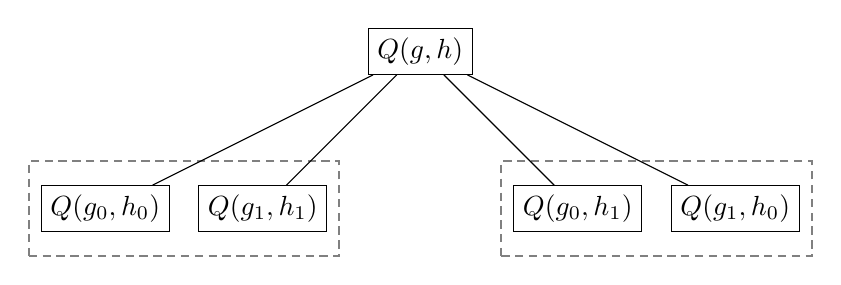
\begin{tikzpicture}[>=stealth]
								\node[draw] (n) at (0,0) {$Q(g,h)$};

								\node[draw] (nl0) at (-4,-2) {$Q(g_0, h_0)$};
								\node[draw] (nl1) at (-2,-2) {$Q(g_1, h_1)$};

								\node[draw] (nr0) at (4,-2) {$Q(g_1, h_0)$};
								\node[draw] (nr1) at (2,-2) {$Q(g_0, h_1)$};

								\node[draw=gray, thick,
									densely dashed,
									inner xsep=1ex, inner ysep=2ex,
									fit=(nl0) (nl1)] {};
								\node[draw=gray, thick,
									densely dashed,
									inner xsep=1ex, inner ysep=2ex,
									fit=(nr0) (nr1)] {};

								\draw[] (nl0) to (n);
								\draw[] (nl1) to (n);
								\draw[] (nr0) to (n);
								\draw[] (nr1) to (n);

							\end{tikzpicture}}}

				In this case
				\begin{multline*}
					\max(\ell_\delta(g_i), \ell_\delta(h_j)) \\
					\leq {\color{OwlYellow}\mu}\cdot (\max(\ell_\delta(g), \ell_\delta(h))+C)
				\end{multline*}

				where
				\emph{$\mu
						=
						0.68142...$}\,.
			\end{framed}
		\end{minipage}
		\begin{minipage}[t]{0.49\linewidth}
			\begin{framed}
				\textbf{\underline{Case 2}:}
				If $g,h\notin \mathrm{Stab}(1)$, then

					{
						\centering

						\medskip

						\resizebox{\linewidth}{!}{
							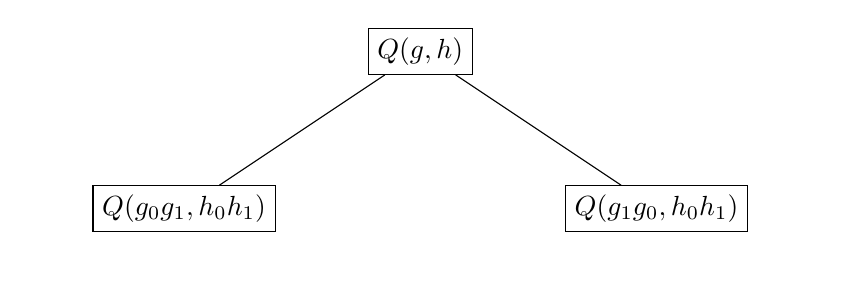
\begin{tikzpicture}[>=stealth]
								\node[draw] (n) at (0,0) {$Q(g,h)$};

								\node[draw] (nl0) at (-3,-2) {$Q(g_0g_1, h_0h_1)$};

								\node[draw] (nr0) at (3,-2) {$Q(g_1g_0, h_0h_1)$};

								\draw[]  (nl0) to (n);
								\draw[]  (nr0) to (n);

								\phantom{
									\node[draw] (n) at (0,0) {$Q(g,h)$};
									\node[draw] (nl0) at (-4,-2) {$Q(g_0, h_0)$};
									\node[draw] (nl1) at (-2,-2) {$Q(g_1, h_1)$};
									\node[draw] (nr0) at (4,-2) {$Q(g_1, h_0)$};
									\node[draw] (nr1) at (2,-2) {$Q(g_0, h_1)$};
									\node[draw=gray, thick,
										densely dashed,
										inner xsep=1ex, inner ysep=2ex,
										fit=(nl0) (nl1)] {};
									\node[draw=gray, thick,
										densely dashed,
										inner xsep=1ex, inner ysep=2ex,
										fit=(nr0) (nr1)] {};
									\draw[] (nl0) to (n);
									\draw[] (nl1) to (n);
									\draw[] (nr0) to (n);
									\draw[] (nr1) to (n);
								}

							\end{tikzpicture}}}

				In this case
				\begin{multline*}
					\max(\ell_\delta(g_a g_b), \ell_\delta(h_c h_d)) \\
					\leq {\color{OwlYellow}\eta}\cdot (\max(\ell_\delta(g), \ell_\delta(h))+\ell_\delta(a))
				\end{multline*}

				where \emph{$\eta=0.8105357...$}\,.
			\end{framed}
		\end{minipage}

		%%%%%%%%%%%%%%%%%%%
	\end{center}

	\pause
	\begin{lemma}
		In any root to leaf path, case~2 can happen \underline{at most} 3 consecutive times.

		Thus, \emph{every 4 levels} we reduce in length by a factor of \emph{$\eta^3\mu$} (up to an additive constant).
	\end{lemma}

	% \textbf{Proof idea}: consider the abelianisation of the words.

\end{frame}
%%%%%%%%%%%%%%%%%%%%%%%%%%%%%%%%%%%%%%%%%%%%%%%%%%%%%%%%%%%%%%%%%%%%%%%%%%
%%%%%%%%%%%%%%%%%%%%%%%%%%%%%%%%%%%%%%%%%%%%%%%%%%%%%%%%%%%%%%%%%%%%%%%%%%

\begin{frame}[t]
	\frametitle{Bringing things together}

	%   \begin{block}{Conclusion}
	%   Let $T$ be the tree associated with $Q(g,h)$.
	%   Then, in any root to leaf path in $T$, the length of our word is reduced by a factor of at least $\eta^3\beta$ after every 4 consecutive steps.
	% \end{block}}

	\begin{lemma}
		The depth of the tree is bound from above by
			{\large\[
					m=
					4\cdot \frac{\log\left(\max(\ell_\delta(g), \ell_\delta(h))/4\right)}{\log(\eta^3\mu)}+C
				\]}
		for some constant $C\geq 0$.
	\end{lemma}

	\begin{lemma}[recall]% (see p.~221 and Prop. 41 on p.~238 of ``Topics in geometric group theory''\nocite{harpe2000}).}
		\vspace{-1ex}
		\[
			[\Grig:\mathrm{Stab}(1)] = 2,\quad
			[\Grig:\mathrm{Stab}(2)] = 8\quad\text{and}\quad
			[\Grig:\mathrm{Stab}(m)] = 2^{5\cdot 2^{m-3}+2}
		\]
		for each $m \geq 3$.\nocite{harpe2000}
	\end{lemma}

	\pause

	From this, we may show that the conjugacy depth of Grigorchuk group is bound from above by
		{\large\[
				\Conj_\Grig(n)
				\preccurlyeq
				e^{n^{\alpha}}
			\]}
	where
		{\large\[
				\alpha
				=
				\frac{-4}{\displaystyle \log_2\left(\eta^3 \beta \right)}
				=
				%2.5873913...\,.
				2.7350028...\,.
			\]}

\end{frame}

%%%%%%%%%%%%%%%%%%%%%%%%%%%%%%%%%%%%%%%%%%%%%%%%%%%%%%%%%%%%%%%%%%%%%%%%%%
%%%%%%%%%%%%%%%%%%%%%%%%%%%%%%%%%%%%%%%%%%%%%%%%%%%%%%%%%%%%%%%%%%%%%%%%%%

\begin{frame}%[standout]
	\centering\Huge{Thanks!}
\end{frame}

\begin{frame}[t,allowframebreaks]
	\frametitle{References}
	\printbibliography[heading=none]
\end{frame}

\end{document}
